%% Introducción sobre Modeling en IR de Baeza
% - Introducción.
% - Taxonomía.
% - Carecterización formal de modelos IR.

\section{Modelo booleano}
	El modelo booleano es el modelo más simple dentro de los que puede implementar un sistema de recuperación de información. Para desarrollarlo, presentamos el siguiente ejemplo. Supongamos que se tiene a disposición las obras del poeta inglés William Shakespear llamada \textbf{Shakespear's Collected Works}. Supongamos también que queremos saber qué obras, dentro de la colección, contiene las palabras Brutus, Caesar pero no Calpurnia. Una forma de resolver la consulta anterior es la siguiente: supongamos que para cada documento (obra dentro de la colección \textbf{Shakespear's Collected Works}) si contiene o no cada una de las palabras que Shakespear utilizó al escribir las obras (Shakespear usó cerca de 32000 palabras diferentes). El resultado es una matriz llamada \textbf{matriz de incidencia término--documento}: $(t, d)$ es igual a 1 si y sólo si el documento en la columna $d$ contiene el término de la fila $t$, y es igual a 0 en caso contrario. La que sigue es parte de la matriz en cuestión tomando el ejemplo de la colección de obras de William Shakespear:
	\begin{quote}
		\[
		\kbordermatrix{
					& Antony \ and \ Cleopatra 	& Julius \ Caesar 	& 	The \ Tempest & 	Hamlet 	& Othello 	& Macbeth 	& ... \\
		Antony		&	1					&		1		&		0		&	0		&	0		&	1		& \\
		Brutus		&	1					&		1		&		0		&	1		&	0		&	0		& \\
		Caesar		&	1					&		1		&		0		&	1		&	1		&	1		& \\
		Calpurnia	&	0					&		1		&		0		&	0		&	0		&	0		& \\
		Cleopatra	&	1					&		0		&		0		&	0		&	0		&	0		& \\
		mercy		&	1					&		0		&		1		&	1		&	1		&	1		& \\
		worser		&	1					&		0		&		1		&	1		&	1		&	0		& \\
		...			&						&				&				&			&			&			&
		}
		\]
	\end{quote}
	
	Dependiendo de la forma en que observamos la matriz término--documento es posible obtener un vector para cada término, el cual indica los documentos en los cuales aparece, ó un vector para cada documento, el cual muestra los términos que ocurren en él. \par
	
	Ahora, resolvamos la consulta del principio; es decir, recuperar todas aquellas obras de la colección que contiene las palabras Brutus, Caesar pero no Calpurnia. Podemos representar ésta consulta de forma booleana, de forma muy simple, de la siguiente manera: \texttt{Brutus AND Caesar AND NOT Calpurnia}. Luego, tomamos los vectores de \texttt{Brutus}, \texttt{Caesar} y el complemento de \texttt{Calpurnia} y los operamos:
	\begin{quote}
		\begin{ttfamily}
			110100 AND 110111 AND 101111 = 100100
		\end{ttfamily}
	\end{quote}
	El resultado anterior nos indica que los documentos los cuales satisfacen la consulta anterior son \textit{Antony and Cleopatra} y \textit{Hamlet}. \par
	
	El \textbf{\textit{modelo booleano}} es un modelo de recuperación de información en el cual podemos plantear cualquier consulta que se encuentre en forma de una expresión booleana de términos; es decir, en la cual los términos estén combinados con operadores AND, OR, y NOT, \cite{manning2009}. El modelo representa a cada documento como un conjunto de palabras.
	
	\subsection{Utilizando un índice invertido}
		Supongamos que tenemos una colección con 1 millón de documentos y que cada documento tenga alrededor de 1000 palabras. Típicamente, habrá alrededor de 500 mil términos distintos en cada uno de éstos documentos. Las dimensiones anteriores varían respecto a diferentes colecciones, pero nos dan una idea de los problemas que tendremos que solucionar utilizando una matriz de incidencia término--documento. Tomando la suposición anterior, debemos construir una matriz término--documento de dimensión 500K $\times$ 1M: ésta posee medio trillón de 0's y 1's, demasiados para caber en la memoria de una computadora estándar. \par
		
		Una representación mucho mejor es sólo recordar los términos que ocurren; es decir, sólo las posiciones 1's. Esto nos lleva a la definición de índice invertido que se desarrolló anteriormente en el Capítulo 2: mantenemos un \textit{diccionario} de términos, luego, para cada término, una lista que guarda en qué documentos el término ocurre. Cada ítem de la lista anterior es llamado \textit{posting}; éste guarda el ID del documento. \par
		
		Para ganar beneficios de rapidez, el sistema de recuperación de información debe contruir el índice invertido antes de que un usuario realice una consulta. Se deben desarrollar los siguientes pasos:
		\begin{enumerate}
			\item Recolectar los documentos a ser indexados.
			\item Convertir cada documento en una lista de tokens (\textit{Tokenization}).
			\item Realizar precedimientos lingüísticos a la lista de tokens del paso 2 (\textit{Normalization}). De ésta forma se obtienen tokens normalizados los cuales, finalmente, serán los términos a indexar.
			\item Indexar aquellos documentos en los cuales ocurren los términos obtenidos en el paso 3 creando un índice invertido.
		\end{enumerate}
		Los pasos 1--3 consisten en el procesamiento de textos que se desarrolló en el capítulo anterior. Mientras que la implementación del índice invertido (paso 4 de la lista anterior) se estudió en el Capítulo 2.
		
		% Figura 1.4 (manning2009)
		
		\subsection{Procesamiento de una consulta booleana}
			Ahora, utilizando índices invertidos como estructura más eficiente para indexar documentos en un sistema de recuperación de información, ¿cómo procesamos una consulta booleana?. Consideremos la siguiente consulta en el modelo booleano sobre el índice invertido presentado en la figura anterior:
			\begin{quote}
				\begin{ttfamily}
					Brutus AND Calpurnia
				\end{ttfamily}
			\end{quote}
			El sistema ejecuta los siguientes pasos:
			\begin{enumerate}
				\item Localizar \texttt{Brutus} en el diccionario de términos.
				\item Devolver sus \textit{postings}.
				\item Localizar \texttt{Calpurnia} en el diccionario de términos.
				\item Devolver sus \textit{postings}.
				\item Intersectar las listas de \textit{postings} de los pasos 2 y 4.
			\end{enumerate}
			Como resultado final, tenemos que la consulta en cuestión se satisface en los documentos 2 y 31 como bien se muestra a continuación:
			\begin{quote}
				\begin{tabular}{lll}
					Brutus & $\longrightarrow$ & \fbox{1}$\rightarrow$\fbox{2}
												$\rightarrow$\fbox{4}
												$\rightarrow$\fbox{11}
												$\rightarrow$\fbox{31}
												$\rightarrow$\fbox{45}
												$\rightarrow$\fbox{173}
												$\rightarrow$\fbox{174} \\
					Calpurnia & $\longrightarrow$ & \fbox{2}$\rightarrow$\fbox{31}
												$\rightarrow$\fbox{54}
												$\rightarrow$\fbox{101} \\
					Intersección & $\Longrightarrow$ & \fbox{2}$\rightarrow$\fbox{31}
				\end{tabular}
			\end{quote}
			
		\subsection{El modelo booleano ante modelos de \textit{ranking} de relevancia}
			Dada una colección de documentos $D$. Sean $d_j \in D$ y $q$ una consulta. Por lo aprendido anteriormente, el documento $d_j$ será relevante ante la consulta $q$ si o sólo si los términos contenidos en la representación del documento en cuestión hacen verdadera a la expresión booleana de la consulta $q$. A lo anterior se lo llama \textit{ranking} de un documento $d_j$ ante una consulta $q$, y lo notamos $R(d_j,q)$. Claramente, es un \textit{ranking} booleano y es la principal desventaja del modelo booleano ante otros modelos de recuperación de información más complejos: las consultas booleanas sólo devuelven un conjunto de documentos el cual no es posible ordenar ya que todos son igual de importantes. \par
			
			Por lo tanto, nos encontramos con un modelo simplista e imposible de satisfacer ciertas necesidades como, por ejemplo:
			\begin{itemize}
				\item Poder escribir consultas en lenguaje natural en vez de en álgebra booleana, la cual sólo tienen conocimientos científicos de la información.
				\item Podríamos tener, también, la necesidad de realizar consultas de \enquote{proximidad} como por ejemplo \texttt{Gates NEAR Microsoft}. Para realizar ésto, el índice tiene que tener la capacidad de capturar proximidades de términos en documentos.
				\item El modelo booleano sólo almacena la presencia o ausencia de un término, pero comúnmente qusieramos acumular evidencia, dando más \enquote{peso} (importancia) a documentos quienes contienen un determinado término varias veces en contraposición a aquellos quienes los contienen una sóla vez. Para realizar ésto debemos tener un método para obtener la frecuencia de un término en un documento en listas de \textit{postings}.
				\item Poder ordenar, en orden de relevancia, los documentos que devuelve el sistema ante una determinada consulta escrita por un usuario.
			\end{itemize}
			
			Las necesidades anteriores se satisfacen en modelos de \textit{ranking} de relevancia como se desarrollarán en las próximas secciones. Es decir, en aquellos modelos de recuperación de información los cuales la función \textit{ranking}, $R$, que emplean no es binaria, como la que emplea el modelo booleano.

\section{Modelo vectorial}

En ciertos contextos el uso de una asignación binaria en la importancia de un documento resulta muy limitante por eso surgió un modelo que permite realizar coincidencias parciales entre una consulta y los documentos de la colección. \\

En este modelo, documentos y consultas se representan mediante vectores t dimensionales, donde t es el número total de términos. Cada componente del vector representa un peso que será asignado al término correspondiente en el documento o la consulta. \\

Formalmente, Sea $k_{i}$ un término indexado del conjunto $V$ de términos, $d_{j}$ un documento en $D$ y $w_{i,j}$  el peso asociado a $(k_{i},d_{j})$ entonces definimos el vector $d_{j}= (w_{1,j}, w_{2,j}, … , w_{t,j})$. De manera análoga se representan las consultas. \\  

Los pesos  asignados a los términos indexados son usados para computar el grado de similitud entre cada documento con la consulta que realiza usuario. Luego se ordenan los documentos recuperados de acuerdo a su relevancia, representada por la distancia entre los vectores de los documentos con el vector de la consulta.\\
\subsection{Ponderación de términos} 

Se asocia un peso a cada término que aparece en el documento $d_{j}$. Si un término no aparece tendrá peso igual a 0. Este peso cuantifica la importancia del término indexado en la descripción del contenido en el documento $d_{j}$.\\

Hay diferentes formas de asignar los pesos teniendo en cuenta que no todos los términos son igualmente descriptivos para un documento.\\

Algunas propiedades de los términos indexados resultan útiles para evaluar su importancia sobre el documento. Para modelos clásicos de IR se suponen que los pesos de los términos son independientes entre sí. En resumen, la cantidad de veces que ocurre un término no está relacionado con la cantidad de veces que pueda aparecer otro.\\

Tomaremos como ejemplo de factor de ponderación de términos: TF-IDF (Frecuencia de término - Frecuencia inversa de documento) es el producto de dos estadísticas que busca reflejar la importancia del término sobre un documento de la colección. Un término es mas importante que otro en un documento si este es más representativo de la información que contiene el documento que aquel. De esta forma, un término es proporcional a la frecuencia con la que ocurre pero ante términos con la misma frecuencia tendrá mayor ponderación el que aparezca en la menor cantidad de documentos, buscando capturar así la idea de especificidad del término. \\

%				\begin{figure}[h]
%					\includegraphics[width=8cm]{tf-idf}
%					\centering
%					\caption{Función de asignación de pesos}
%				\end{figure}

\subsection{Función de ranking}

Tomando el esquema de asignación de ponderación TF-IDF, el peso de cada término influirá en el ranking de documentos de acuerdo a su especificidad. \\ 

Dada una consulta y un documento con una única coincidencia pero en un término de mayor peso, éste podría darle más valor de ranking que otro documento con varias coincidencias en términos de menores peso. \\

Entonces podemos calcular la similitud entre dos documentos o entre un documento y una consulta como el coseno del ángulo formado por los vectores representativos de cada documento dj y consulta q. 

				\begin{figure}[h]
					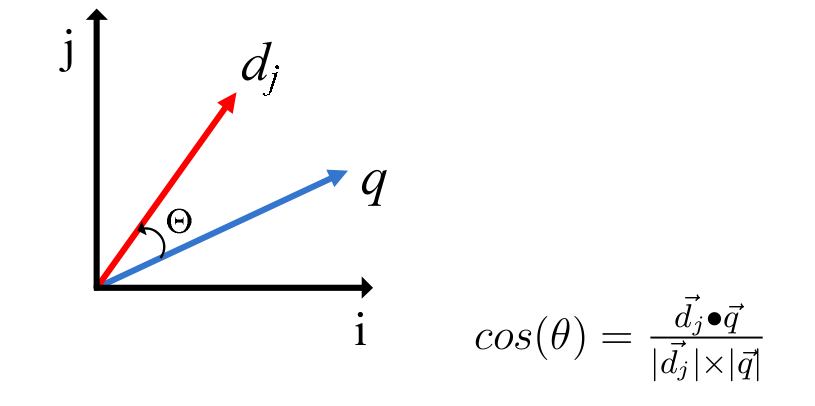
\includegraphics[width=8cm]{vector-distance}
					\centering
					\caption{Calcular la similitud}
				\end{figure}


\section{Modelo probabilístico}

Este modelo intenta resolver el problema de la recuperación de información estimando la probabilidad de que un documento sea relevante ante una determinada consulta.\\
Se representa a los documentos como vectores de incidencia de términos. Inicialmente se asignan pesos binarios a los términos de acuerdo a si está presente o no en el documento.\\
Se supone que existe para cada consulta un conjunto de respuesta ideal $R$ que satisface la consulta, no se lo conoce de antemano pero se va refinando consulta tras consulta.\\
La consulta inicial del usuario permite al sistema responder con un primer conjunto de respuesta. Luego el usuario inspeccionará algunos documentos y el sistema utilizará esa información para mejorar la descripción del conjunto de respuesta. Iterando este procedimiento se espera obtener una caracterización lo mas parecida a la que descripción del conjunto de respuesta ideal.\\
Para este modelo se asume la hipótesis del principio de probabilidad donde dada una consulta $q$ y un documento $d_{j}$, el modelo probabilístico estimará la probabilidad que el usuario encuentre relevante al documento $d_{j}$ asumiendo que la probabildad de relevancia sólo depende de la consulta y la representación del documento en el modelo.\\

\subsection{Funcion de ranking}

Como ya dijimos, la ponderación de los términos indexados es binaria, es decir, $w_{i,j} /in {0,1}$.
Sea $R$ el conjunto de respuesta conocido como relevante para la consulta del usuario. Definimos $\overline{R}$ como el complemento de $R$ y sea $P(R|d_{j})$ la probabilidad que el documento $d_{j}$ resulte relevante a la consulta $q$ y $P(\overline{R}|d_{j})$ la probabildad de que $d_{j}$ no sea relevante a la consulta $q$.\\
La similaridad entre el documento $d_{j}$ y la consulta $q$ queda definida por la función:
			\begin{figure}[h]
					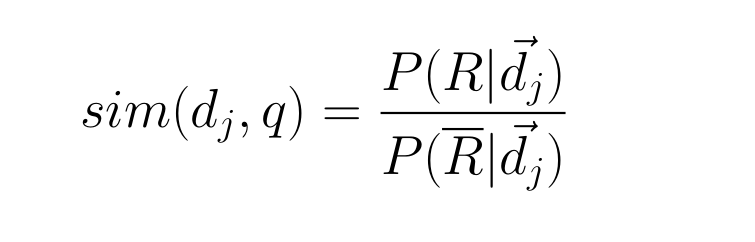
\includegraphics[width=8cm]{prob-sim}
					\centering
					\caption{Calcular la similitud}
				\end{figure}
				
Usando la regla de Bayes y sabiendo que $P(R)$ y $P(\overline{R})$ valen lo mismo para todos los documentos de la colección:
			\begin{figure}[h]
					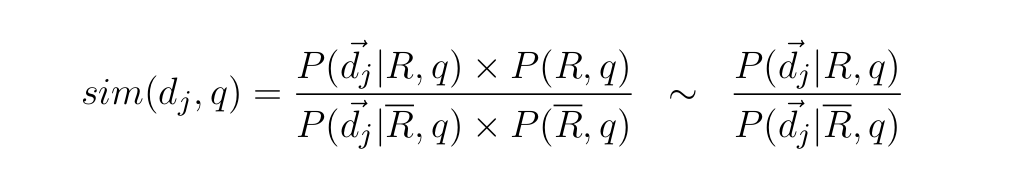
\includegraphics[width=8cm]{prob-sim2}
					\centering
					\caption{Calcular la similitud}
				\end{figure}
				


\section{Comparación entre modelos}

Partiendo del modelo booleano que es el más simple pero también pobre porque no tiene la habilidad de realizar coincidencias parciales lo que define una baja performance del sistema respecto de los otro dos modelos.
En cuanto a los últimos dos modelos, como se menciona en \cite{baeza1999}, Croft sugiere que el modelo de probabilidades aporta un mejor rendimiento de recuperación. Sin embargo, se demostró que el rendimiento del modelo vectorial supera a los demás para colecciones de documentos más generales.
En cuanto a la desventaja que se observa en estos modelos es que se asume independecia entre los términos.